% Biên dịch bằng XeLaTeX (Overleaf: Menu -> Compiler -> XeLaTeX)
\documentclass[conference]{IEEEtran}
\usepackage{fontspec}
\setmainfont{TeX Gyre Termes}          % tương đương Times, đủ dấu tiếng Việt
\usepackage{polyglossia}
\setdefaultlanguage{vietnamese}
\usepackage{amsmath,amssymb}
\usepackage{graphicx}
\usepackage{booktabs}
\usepackage{multirow}
\usepackage{tikz}
\usetikzlibrary{arrows.meta,positioning,shapes.geometric}
\usepackage{cite}
\usepackage{url}

% Ô đánh dấu chỗ còn chờ số liệu thật
\newcommand{\todo}[1]{\textbf{[#1]}}

\begin{document}

\title{Chấm điểm an toàn phòng thí nghiệm từ ảnh: so sánh hệ thống dựa trên luật và mô hình ngôn ngữ--thị giác với đánh giá của con người}

\author{
\IEEEauthorblockN{Trần Tuấn Kiệt \quad Lành Diệu Hương \quad Lê Quốc Dũng}
\IEEEauthorblockA{Học viện Công nghệ Bưu chính Viễn thông\\
kiett9467@gmail.com, dieuhuong1027@gmail.com, lequocdungcv@gmail.com}
}

\maketitle

% =====================================================================
\begin{abstract}
Việc kiểm tra điều kiện an toàn phòng thí nghiệm hiện chủ yếu được thực hiện thủ công, tốn nhân lực và phụ thuộc vào người đánh giá. Bài báo khảo sát mức độ khớp giữa hai hướng chấm điểm tự động và đánh giá của con người trên bốn tiêu chí gọn gàng, vệ sinh và an toàn: vật cản trên lối đi, vật dụng cá nhân trên bàn thí nghiệm, bình chữa cháy bị che khuất và đồ ăn uống trong khu vực thí nghiệm. Hướng thứ nhất là hệ thống dựa trên luật, kết hợp mô hình phát hiện đối tượng YOLO với các luật quan hệ không gian theo vùng chức năng. Hướng thứ hai là mô hình ngôn ngữ--thị giác (VLM) được yêu cầu chấm điểm trực tiếp mà không huấn luyện, với ba biến thể prompt. Trên bộ 62 ảnh tự thu thập tại một phòng thí nghiệm điện tử, được ba người chấm độc lập (Fleiss' $\kappa$ từ 0{,}69 đến 0{,}98), hệ thống dựa trên luật khớp với người chấm tốt hơn ở hai tiêu chí phụ thuộc vị trí: vật cản lối đi ($\kappa = 0{,}74$ so với $0{,}44$) và bình chữa cháy bị che ($0{,}90$ so với $0{,}78$). Ngược lại, VLM vượt trội ở hai tiêu chí đòi hỏi nhận biết loại đồ vật: vật dụng cá nhân ($0{,}88$ so với $0{,}58$) và đồ ăn uống ($0{,}97$ so với $0{,}78$). Kết quả của VLM thay đổi đáng kể theo cách diễn đạt prompt ở tiêu chí lối đi và vật dụng cá nhân. Hai hướng có điểm mạnh bù trừ nhau, gợi ý một hệ thống kết hợp theo từng tiêu chí.
\end{abstract}

\begin{IEEEkeywords}
an toàn phòng thí nghiệm, phát hiện đối tượng, YOLO, mô hình ngôn ngữ--thị giác, độ đồng thuận, hệ số kappa
\end{IEEEkeywords}

% =====================================================================
\section{Giới thiệu}

Phòng thí nghiệm tại các trường đại học hiện được kiểm tra điều kiện an toàn chủ yếu bằng phương pháp thủ công: cán bộ phụ trách quan sát trực tiếp và đối chiếu với một bảng kiểm. Cách làm này có ba hạn chế: (i) tốn nhân lực nên không thể thực hiện thường xuyên khi số lượng phòng lớn; (ii) kết quả phụ thuộc vào người đánh giá, thiếu nhất quán giữa các lần kiểm tra; (iii) không lưu lại bằng chứng có hệ thống để theo dõi mức độ cải thiện theo thời gian. Trong khi đó, camera giám sát đã được lắp đặt phổ biến, đặt ra câu hỏi liệu có thể tận dụng nguồn hình ảnh sẵn có để tự động hóa một phần công việc đánh giá hay không, và nếu có thì mức độ tin cậy đạt đến đâu.

Các nghiên cứu hiện có về giám sát an toàn phòng thí nghiệm bằng thị giác máy tính tập trung chủ yếu vào phát hiện trang bị bảo hộ cá nhân~\cite{ali2022yolov5,ppe2024safety,yolov7ppe2024}. Việc đánh giá điều kiện gọn gàng, vệ sinh và an toàn ở mức toàn cảnh của căn phòng ít được nghiên cứu định lượng. Song song đó, mô hình ngôn ngữ--thị giác (Vision-Language Model, VLM) mở ra khả năng chấm điểm trực tiếp từ mô tả tiêu chí mà không cần huấn luyện, nhưng các nghiên cứu gần đây cho thấy hướng này còn kém ổn định~\cite{goyal2026zeroshot,weng2026prompt,abdullah2025isafetybench,yarrabothula2026steelbench}.

Bài báo trả lời ba câu hỏi nghiên cứu:
\begin{itemize}
  \item \textbf{RQ1:} Kết quả chấm điểm tự động khớp với người chấm ở mức nào, xét riêng từng tiêu chí?
  \item \textbf{RQ2:} Giữa hệ thống dựa trên luật và VLM, hướng nào gần với người chấm hơn, và với tiêu chí nào?
  \item \textbf{RQ3:} Kết quả của VLM có ổn định khi thay đổi cách diễn đạt prompt hay không?
\end{itemize}

Đóng góp của bài báo gồm: (1) một bảng tiêu chí nhị phân có định nghĩa định lượng cho bốn tiêu chí an toàn phòng thí nghiệm; (2) một hệ thống chấm điểm dựa trên luật quan hệ không gian, sử dụng các mô hình phát hiện huấn luyện trên dữ liệu công khai và đánh giá trên ảnh phòng thí nghiệm thực tế (khác miền dữ liệu); (3) một thiết kế đánh giá ba cột đối chiếu hệ thống luật, VLM và người chấm, kèm phân tích ca lỗi.

% =====================================================================
\section{Các nghiên cứu liên quan và cơ sở lý thuyết}

\subsection{Giám sát an toàn phòng thí nghiệm bằng phát hiện đối tượng}
Ali và cộng sự~\cite{ali2022yolov5} xây dựng hệ thống giám sát an toàn phòng thí nghiệm giáo dục bằng YOLOv5 và YOLOv7 trên 481 ảnh tự thu thập, đạt mAP cao nhất 77{,}40\%. Nghiên cứu~\cite{ppe2024safety} so sánh YOLOv4, YOLOv5 và YOLOv6 trong phát hiện việc sử dụng trang bị bảo hộ tại phòng thực hành chế tạo, đạt mAP 0{,}757 với YOLOv5. Nghiên cứu~\cite{yolov7ppe2024} cải tiến YOLOv7 cho bài toán tương tự. Các công trình này đều tập trung vào \emph{con người} (có đeo bảo hộ hay không) thay vì \emph{trạng thái của không gian} (lối đi, mặt bàn, thiết bị phòng cháy).

\subsection{Mô hình ngôn ngữ--thị giác trong đánh giá an toàn}
Bộ chuẩn iSafetyBench~\cite{abdullah2025isafetybench} gồm 1.100 video công nghiệp cho thấy tám mô hình video--ngôn ngữ ở chế độ không huấn luyện gặp khó khăn rõ rệt khi nhận diện hoạt động nguy hiểm. SteelBench~\cite{yarrabothula2026steelbench} ghi nhận rằng ngay cả khi nhận dạng đúng hành động, 37--58\% trường hợp vẫn cho phán đoán an toàn sai. Goyal và cộng sự~\cite{goyal2026zeroshot} chỉ ra hiện tượng sụp đổ lớp (85--100\% dự đoán rơi vào một mức) và độ nhạy với prompt lên tới 32 điểm phần trăm trên cùng một ảnh. Weng và cộng sự~\cite{weng2026prompt} cho thấy các prompt tương đương về ngữ nghĩa có thể cho xác suất khác nhau đáng kể. Theo khảo sát của nhóm, chưa có nghiên cứu nào so sánh trực tiếp VLM với hệ thống dựa trên luật và với người chấm trong bối cảnh đánh giá toàn cảnh phòng thí nghiệm.

\subsection{Đo độ đồng thuận}
Với hai nguồn đánh giá trên cùng $N$ mẫu, hệ số Cohen's kappa hiệu chỉnh phần đồng thuận do ngẫu nhiên:
\begin{equation}
  \kappa = \frac{p_o - p_e}{1 - p_e},
  \label{eq:cohen}
\end{equation}
trong đó $p_o$ là tỷ lệ khớp quan sát được và $p_e$ là tỷ lệ khớp kỳ vọng nếu hai nguồn độc lập. Với $m \ge 2$ người chấm, nhóm sử dụng Fleiss' kappa~\cite{fleiss1971}:
\begin{equation}
  \kappa_F = \frac{\bar{P} - \bar{P}_e}{1 - \bar{P}_e},\quad
  \bar{P} = \frac{1}{N}\sum_{i=1}^{N}\frac{\sum_j n_{ij}^2 - m}{m(m-1)},
  \label{eq:fleiss}
\end{equation}
với $n_{ij}$ là số người xếp mẫu $i$ vào lớp $j$ và $\bar{P}_e = \sum_j p_j^2$. Giá trị $\kappa$ được diễn giải theo thang của Landis và Koch~\cite{landis1977}: $0{,}21$--$0{,}40$ khá, $0{,}41$--$0{,}60$ trung bình, $0{,}61$--$0{,}80$ đáng kể, trên $0{,}80$ gần như hoàn hảo.

% =====================================================================
\section{Phương pháp đề xuất}

\subsection{Thiết kế nghiên cứu}
Cùng một bộ ảnh được đánh giá độc lập bởi ba nguồn (Hình~\ref{fig:design}): (1) người chấm, dùng làm mốc chuẩn; (2) hệ thống dựa trên luật; (3) VLM. Ảnh thử nghiệm \emph{không} được dùng để huấn luyện bất kỳ mô hình nào.

\begin{figure}[t]
\centering
\begin{tikzpicture}[node distance=4mm and 6mm, font=\scriptsize,
  box/.style={draw, rounded corners=2pt, align=center, minimum height=6mm, text width=19mm},
  arr/.style={-{Stealth[length=1.6mm]}}]
  \node[box] (img) {Ảnh phòng\\thí nghiệm};
  \node[box, right=of img, yshift=9mm] (h) {Người chấm\\(đa số)};
  \node[box, right=of img] (r) {YOLO +\\bộ luật};
  \node[box, right=of img, yshift=-9mm] (v) {VLM\\(3 prompt)};
  \node[box, right=of r, text width=16mm] (cmp) {So sánh từng\\tiêu chí ($\kappa$)};
  \foreach \n in {h,r,v} { \draw[arr] (img.east) -- (\n.west); \draw[arr] (\n.east) -- (cmp.west); }
\end{tikzpicture}
\caption{Thiết kế đánh giá ba cột.}
\label{fig:design}
\end{figure}

\subsection{Bảng tiêu chí}
Mỗi tiêu chí được chấm nhị phân: Đạt (0) hoặc Vi phạm (1). Định nghĩa đầy đủ được trình bày trong Bảng~\ref{tab:rubric}. Bản đề cương ban đầu dự kiến thang ba mức và sáu tiêu chí. Nhóm thu hẹp còn bốn tiêu chí nhị phân để (i) giảm tính chủ quan khi gán nhãn và (ii) loại hai tiêu chí khó phát hiện bằng ảnh (hóa chất ngoài tủ, dây điện cắt ngang lối đi), hai tiêu chí này được để lại cho hướng phát triển.

\begin{table}[t]
\centering
\caption{Bảng tiêu chí và luật máy tương ứng}
\label{tab:rubric}
\footnotesize
\begin{tabular}{p{0.9cm}p{3.3cm}p{3.1cm}}
\toprule
Tiêu chí & Vi phạm khi & Luật máy \\
\midrule
C1 Lối đi & Có vật cỡ từ balo trở lên đặt trên sàn trong lối đi & $R \ge \tau_1$ (Mục~\ref{sec:rules}) \\
C2 Đồ cá nhân & $\ge 3$ vật dụng cá nhân trên mặt bàn thí nghiệm & Đếm vật có tâm trong vùng bàn $\ge 3$ \\
C3 Bình chữa cháy & Bị che $\ge 1/3$, khó tiếp cận, hoặc không còn ở vị trí & Không phát hiện bình, hoặc $V < \tau_v$, hoặc $O \ge \tau_o$ \\
C4 Đồ ăn uống & Có bất kỳ đồ ăn, đồ uống nào (không tính dụng cụ thí nghiệm) & Có $\ge 1$ đối tượng thuộc nhóm đồ ăn uống \\
\bottomrule
\end{tabular}
\end{table}

\subsection{Hệ thống dựa trên luật}
\label{sec:rules}
Hệ thống gồm ba bộ phát hiện và một bộ luật (Hình~\ref{fig:rules}):
\begin{itemize}
  \item \textbf{YOLO11 huấn luyện sẵn trên COCO}~\cite{lin2014coco,ultralytics}: nhận dạng ghế, balo, túi, vali, cốc, chai, bát, thực phẩm, điện thoại, laptop, sách.
  \item \textbf{YOLO11 tinh chỉnh} trên bộ dữ liệu công khai Fire-ART~\cite{wen2025fireart} để phát hiện bình chữa cháy, lớp không có trong COCO.
  \item \textbf{YOLO-World}~\cite{cheng2024yoloworld} ở chế độ từ vựng mở để phát hiện thùng carton, cũng là lớp không có trong COCO.
\end{itemize}
Với mỗi góc camera cố định, ba vùng chức năng được khoanh một lần bằng đa giác: lối đi $A$, mặt bàn $B$ và vị trí bình chữa cháy $Z$. Đây là cấu hình một lần cho mỗi camera, tương tự cách thiết lập vùng trong hệ thống giám sát thực tế.

\begin{figure}[t]
\centering
\begin{tikzpicture}[node distance=3mm, font=\scriptsize,
  box/.style={draw, rounded corners=2pt, align=center, text width=40mm, minimum height=5mm},
  arr/.style={-{Stealth[length=1.6mm]}}]
  \node[box] (s1) {Bước 1: Đọc ảnh, xác định góc camera};
  \node[box, below=of s1] (s2) {Bước 2: Phát hiện đối tượng\\(COCO + bình chữa cháy + thùng)};
  \node[box, below=of s2] (s3) {Bước 3: Nạp đa giác vùng $A$, $B$, $Z$};
  \node[box, below=of s3] (s4) {Bước 4: Tính $R$, $n_B$, $V$, $O$, $n_F$};
  \node[box, below=of s4] (s5) {Bước 5: So ngưỡng $\Rightarrow$ C1--C4};
  \foreach \a/\b in {s1/s2,s2/s3,s3/s4,s4/s5} \draw[arr] (\a) -- (\b);
\end{tikzpicture}
\caption{Lưu đồ hệ thống dựa trên luật.}
\label{fig:rules}
\end{figure}

\textbf{C1 -- Tỷ lệ chiếm dụng lối đi.} Gọi $B_i^{\text{đáy}}$ là phần đáy (25\% chiều cao) của hộp bao vật cản thứ $i$, xấp xỉ diện tích tiếp xúc với sàn. Tỷ lệ chiếm dụng là
\begin{equation}
  R = \frac{\left|\left(\bigcup_i B_i^{\text{đáy}}\right) \cap A\right|}{|A|}.
  \label{eq:R}
\end{equation}
Phép hợp $\bigcup$ đảm bảo phần diện tích chồng lấn giữa các vật không bị tính hai lần. Tiêu chí vi phạm khi $R \ge \tau_1$, với $\tau_1 = 5\%$ được chọn trước khi thu thập dữ liệu, tương ứng một vật cỡ balo trên lối đi điển hình.

\textbf{Ví dụ tính tay.} Trên lưới $10\times10$ ô, lối đi $A$ gồm các ô từ $(3,1)$ đến $(7,10)$, diện tích $|A| = 5\times10 = 50$ ô. Để minh họa, dùng cả hộp bao và ngưỡng $15\%$:
\begin{itemize}
  \item Vật cản tại ô $(4,2)$--$(6,4)$, diện tích $9$ ô, nằm trọn trong $A$: $R = 9/50 = 18\% \ge 15\%$, kết luận \emph{vi phạm}.
  \item Vật cản nhỏ tại ô $(4,2)$--$(5,3)$, diện tích $4$ ô: $R = 4/50 = 8\% < 15\%$, kết luận \emph{đạt}.
  \item Vật cản tại ô $(1,5)$--$(4,8)$, diện tích $16$ ô, chỉ cột 3--4 (8 ô) nằm trong $A$: $R = 8/50 = 16\%$, kết luận \emph{vi phạm}. Phần nằm ngoài lối đi không được tính.
\end{itemize}
Cả ba ví dụ được đưa vào bộ kiểm thử tự động của hệ thống.

\textbf{C2 -- Vật dụng cá nhân.} $n_B$ là số đối tượng thuộc nhóm vật dụng cá nhân có tâm hộp bao nằm trong $B$. Tiêu chí vi phạm khi $n_B \ge 3$.

\textbf{C3 -- Bình chữa cháy.} Gọi $E$ là hợp các hộp bao bình chữa cháy giao với $Z$, và $Q$ là hợp các hộp bao của vật có thể che (balo, túi, ghế, thùng\ldots). Ta tính tỷ lệ nhìn thấy và tỷ lệ bị che:
\begin{equation}
  V = \frac{|E \cap Z|}{|Z|}, \qquad O = \frac{|Q \cap Z|}{|Z|}.
  \label{eq:VO}
\end{equation}
Tiêu chí vi phạm khi không phát hiện được bình, hoặc $V < \tau_v = 0{,}5$, hoặc $O \ge \tau_o = 1/3$.

\textbf{C4 -- Đồ ăn uống.} $n_F$ là số đối tượng thuộc nhóm đồ ăn uống của COCO (cốc, chai, ly, bát, trái cây, bánh\ldots). Tiêu chí vi phạm khi $n_F \ge 1$. Do COCO gộp chai nước uống và chai hóa chất chung lớp \emph{bottle}, luật này dự kiến sinh báo động giả. Bộ ảnh được thiết kế có chủ đích các tình huống như vậy để phân tích.

\subsection{Mô hình ngôn ngữ--thị giác}
Ảnh được thu nhỏ về cạnh dài 1568 điểm ảnh và gửi kèm prompt tiếng Anh mô tả bốn tiêu chí qua API của Gemini, phiên bản \texttt{gemini-3.5-flash}, chạy trong hai ngày 8--9/10/2026. Nhiệt độ lấy mẫu đặt bằng 0, đầu ra bắt buộc ở dạng JSON. Ba biến thể prompt được sử dụng: \textbf{P1} chi tiết, có định nghĩa đầy đủ như Bảng~\ref{tab:rubric}; \textbf{P2} rút gọn, mỗi tiêu chí một dòng; \textbf{P3} giống P1 nhưng đảo thứ tự tiêu chí (C4, C3, C2, C1). Mô hình không được huấn luyện hay cung cấp ví dụ.

\subsection{Người chấm}
Ba người chấm, không tham gia dàn dựng ảnh và không biết kịch bản của từng ảnh, chấm độc lập theo bảng tiêu chí. Trước khi chấm, mỗi người đọc bản hướng dẫn kèm ảnh tham khảo vị trí bình chữa cháy của từng góc chụp. Phiếu chấm chỉ cho phép nhập 0 hoặc 1, thứ tự ảnh được xáo trộn khác nhau cho mỗi người. Nhãn chuẩn của mỗi ảnh là nhãn đa số. Độ đồng thuận giữa người chấm (Fleiss' $\kappa$) được dùng làm giới hạn trên tham chiếu cho độ khớp của máy.

% =====================================================================
\section{Thực nghiệm và kết quả}

\subsection{Dữ liệu}
\textbf{Dữ liệu huấn luyện.} Mô hình bình chữa cháy được tinh chỉnh trên Fire-ART~\cite{wen2025fireart} (15 lớp thiết bị phòng cháy, giấy phép CC BY 4.0). Nhóm sử dụng phần ảnh được phát hành trực tiếp (1.174 ảnh), chỉ giữ lớp bình chữa cháy và chuyển nhãn đa giác thành hộp bao. Kết quả gồm 179 ảnh có bình (207 đối tượng) và 179 ảnh âm chọn ngẫu nhiên từ các ảnh không có bình, chia ngẫu nhiên thành 287 ảnh huấn luyện và 71 ảnh kiểm định. Mô hình YOLO11n khởi tạo từ trọng số COCO, huấn luyện ở độ phân giải 640, batch 8, trên GPU NVIDIA GeForce MX350 (2~GB), với cơ chế dừng sớm sau 10 epoch không cải thiện. Quá trình huấn luyện dừng ở epoch 46, mô hình tốt nhất ở epoch 36, đạt trên tập kiểm định mAP@0{,}5 = 0{,}797, mAP@0{,}5:0{,}95 = 0{,}514, precision 0{,}876 và recall 0{,}672.

\textbf{Dữ liệu thử nghiệm.} Do Học viện không có phòng thí nghiệm hóa học, nhóm thu thập dữ liệu tại một phòng thí nghiệm điện tử. Tổng cộng 62 ảnh được chụp bằng điện thoại từ ba vị trí đặt máy; hai vị trí được chụp thêm ở nhiều độ cao, tạo thành sáu góc chụp với 5--13 ảnh mỗi góc. Ở mỗi góc, các vật dụng (ghế, balo, áo khoác, sách vở, chai nước\ldots) được sắp xếp theo các kịch bản khác nhau, kể cả ảnh ``bẫy'' chứa vật dễ gây nhầm. Ảnh không chứa người. Với phòng thí nghiệm điện tử, thiết bị đo, bộ nguồn, mỏ hàn, bo mạch và chai dung dịch vệ sinh mạch không được tính là vật dụng cá nhân hay đồ uống. Theo nhãn đa số, số ảnh vi phạm của C1--C4 lần lượt là 32, 11, 32 và 26 trên 62. Như vậy C1, C3, C4 tương đối cân bằng, còn C2 có ít ca vi phạm.

Các vùng chức năng được một thành viên vẽ một lần cho mỗi góc chụp bằng công cụ trên trình duyệt. Sáu ảnh bị lệch khung so với ảnh khác cùng góc được vẽ vùng riêng.

\subsection{Độ đồng thuận giữa người chấm}
Bảng~\ref{tab:inter} cho thấy người chấm đồng thuận gần như hoàn hảo ở C1, C3, C4 ($\kappa_F \ge 0{,}89$) và ở mức đáng kể ở C2 ($\kappa_F = 0{,}69$). Bất đồng ở C2 chủ yếu xuất phát từ việc xác định một vật có phải đồ cá nhân hay không (ví dụ áo khoác vắt trên ghế cạnh bàn) và ngưỡng đếm ba vật. Mức đồng thuận cao cho thấy bảng tiêu chí đủ rõ để dùng nhãn đa số làm mốc chuẩn.

\begin{table}[t]
\centering
\caption{Độ đồng thuận giữa ba người chấm ($N = 62$)}
\label{tab:inter}
\footnotesize
\begin{tabular}{lccc}
\toprule
Tiêu chí & Fleiss $\kappa$ & Cohen $\kappa$ TB & Cả ba khớp \\
\midrule
C1 Lối đi & 0{,}89 & 0{,}89 & 92\% \\
C2 Đồ cá nhân & 0{,}69 & 0{,}70 & 85\% \\
C3 Bình chữa cháy & 0{,}98 & 0{,}98 & 98\% \\
C4 Đồ ăn uống & 0{,}96 & 0{,}96 & 97\% \\
\bottomrule
\end{tabular}
\end{table}

\subsection{So sánh hệ thống luật và VLM với người chấm (RQ1, RQ2)}
Bảng~\ref{tab:main} và Hình~\ref{fig:kappa} so sánh hai hệ thống với nhãn đa số. Khoảng tin cậy 95\% của $\kappa$ được ước lượng bằng bootstrap 2.000 lần.

\begin{table}[t]
\centering
\caption{Độ khớp với nhãn đa số của người chấm ($N = 62$). FP: báo động giả, FN: bỏ sót}
\label{tab:main}
\footnotesize
\setlength{\tabcolsep}{3.5pt}
\begin{tabular}{llcccc}
\toprule
 & Tiêu chí & Khớp & $\kappa$ [CI 95\%] & F1 & FP/FN \\
\midrule
\multirow{4}{*}{Luật} & C1 & 87\% & \textbf{0{,}74} [0{,}56; 0{,}90] & 0{,}88 & 6/2 \\
 & C2 & 90\% & 0{,}58 [0{,}22; 0{,}85] & 0{,}62 & 0/6 \\
 & C3 & 95\% & \textbf{0{,}90} [0{,}77; 1{,}00] & 0{,}95 & 2/1 \\
 & C4 & 89\% & 0{,}78 [0{,}61; 0{,}90] & 0{,}88 & 7/0 \\
\midrule
\multirow{4}{*}{VLM P1} & C1 & 73\% & 0{,}44 [0{,}25; 0{,}65] & 0{,}78 & 16/1 \\
 & C2 & 97\% & \textbf{0{,}88} [0{,}68; 1{,}00] & 0{,}90 & 0/2 \\
 & C3 & 89\% & 0{,}78 [0{,}61; 0{,}90] & 0{,}88 & 0/7 \\
 & C4 & 98\% & \textbf{0{,}97} [0{,}90; 1{,}00] & 0{,}98 & 1/0 \\
\bottomrule
\end{tabular}
\end{table}

\begin{figure}[t]
\centering
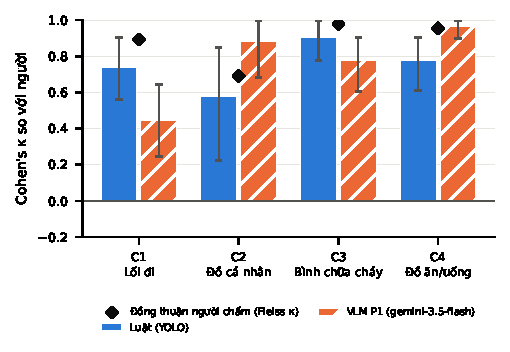
\includegraphics[width=\columnwidth]{fig_kappa.pdf}
\caption{Cohen's $\kappa$ của hai hệ thống so với người chấm theo từng tiêu chí (thanh lỗi: CI 95\%). Điểm đen: Fleiss' $\kappa$ giữa người chấm.}
\label{fig:kappa}
\end{figure}

\textbf{RQ1.} Cả hai hệ thống đều đạt mức khớp từ trung bình trở lên ($\kappa \ge 0{,}44$) ở mọi tiêu chí. Ở tiêu chí tốt nhất của mỗi hệ thống, độ khớp tiệm cận mức đồng thuận giữa người với người: luật đạt $\kappa = 0{,}90$ ở C3 (người: 0{,}98), VLM đạt $0{,}97$ ở C4 (người: 0{,}96).

\textbf{RQ2.} Hai hướng có điểm mạnh bù trừ nhau. Hệ thống luật tốt hơn ở hai tiêu chí phụ thuộc \emph{vị trí}: C1 (0{,}74 so với 0{,}44) và C3 (0{,}90 so với 0{,}78). Nhờ vùng chức năng được khoanh trước, luật biết chính xác đâu là lối đi và đâu là chỗ đặt bình. VLM tốt hơn ở hai tiêu chí phụ thuộc \emph{loại đồ vật}: C2 (0{,}88 so với 0{,}58) và C4 (0{,}97 so với 0{,}78), nhờ nhận biết được những vật không có trong 80 lớp COCO như áo khoác, ví, và phân biệt được chai nước với vật có hình dạng giống chai. Do khoảng tin cậy còn chồng lấn với $N = 62$, các chênh lệch này cần được kiểm chứng trên dữ liệu lớn hơn, ngoại trừ C1 và C4 nơi chênh lệch đã khá rõ.

\subsection{Độ ổn định của VLM theo prompt (RQ3)}
Do giới hạn hạn mức của API miễn phí, P2 và P3 chỉ được chạy trên 33 ảnh đầu tiên theo thứ tự tên tệp, trong khi P1 chạy trên đủ 62 ảnh. Trên 33 ảnh chung (Bảng~\ref{tab:prompt}), VLM ổn định hoàn toàn ở C4 và gần như hoàn toàn ở C3, nhưng thay đổi rõ ở C1 và C2: chỉ 70\% và 76\% số ảnh được ba prompt cho cùng kết luận. Prompt rút gọn P2 kém nhất: $\kappa$ so với người chấm ở C2 giảm còn 0{,}20 (P1: 0{,}88), do P2 không liệt kê rõ những gì được tính, nên mô hình đếm cả chai nước và gói bánh là vật dụng cá nhân (7 trên 10 ca sai là báo động giả). Đảo thứ tự tiêu chí (P3) không làm giảm chất lượng. Kết quả này phù hợp với nhận định của~\cite{goyal2026zeroshot,weng2026prompt}: định nghĩa chi tiết trong prompt quan trọng hơn thứ tự trình bày.

\begin{table}[t]
\centering
\caption{Độ ổn định của VLM giữa ba prompt (33 ảnh chung). Đồng nhất: tỷ lệ ảnh được cả ba prompt cho cùng kết luận}
\label{tab:prompt}
\footnotesize
\begin{tabular}{lccc}
\toprule
Tiêu chí & Đồng nhất & $\kappa_F$ giữa prompt & Khớp người \\
\midrule
C1 & 70\% & 0{,}49 & 64--82\% \\
C2 & 76\% & 0{,}46 & 73--97\% \\
C3 & 97\% & 0{,}96 & 88--91\% \\
C4 & 100\% & 1{,}00 & 100\% \\
\bottomrule
\end{tabular}
\end{table}

\subsection{Phân tích ca lỗi}
\textbf{Bình chữa cháy bị nhận thành chai (luật, C4).} Sáu trên bảy ca báo động giả C4 của hệ thống luật có cùng nguyên nhân: mô hình COCO nhận chính bình chữa cháy màu đỏ thành lớp \emph{bottle} (khung trùng với khung bình, IoU 0{,}50--0{,}95), dẫn đến kết luận ``có đồ uống'' (Hình~\ref{fig:errors}a). Lỗi này cũng giải thích vì sao cần mô hình bình chữa cháy riêng: mô hình huấn luyện sẵn không có lớp này nên gán vật thể vào lớp gần nhất về hình dạng.

\textbf{Áo khoác, điểm mù của COCO (luật, C1--C3).} COCO không có lớp áo khoác nên: áo trùm lên bình chữa cháy không được tính là vật che, dẫn đến bỏ sót C3 (Hình~\ref{fig:errors}b); ghế có áo vắt lên bị nhận thành \emph{person} và bị luật bỏ qua theo quy tắc ``không tính người'', dẫn đến bỏ sót C1; áo và ví trên bàn không được đếm, dẫn đến sáu ca bỏ sót C2.

\textbf{VLM quá khắt khe ở lối đi (C1).} 16 ca báo động giả C1 của VLM phần lớn do mô hình coi ghế, balo cạnh bàn hoặc loa và khung kim loại kê sát tường là vật cản, trong khi người chấm xác định các vật này nằm ngoài lối đi. Không có thông tin vùng, VLM không phân biệt được vật đặt đúng chỗ với vật lấn ra lối đi.

\textbf{VLM bỏ sót bình bị che (C3).} Trong 7 ca bỏ sót C3, có 4 ca VLM giải thích ``không thấy bình chữa cháy nên không vi phạm'', trong khi theo tiêu chí, việc không còn nhìn thấy bình ở vị trí quy định chính là vi phạm. Đây là hạn chế khi VLM không biết trước vị trí chuẩn của bình.

\begin{figure}[t]
\centering
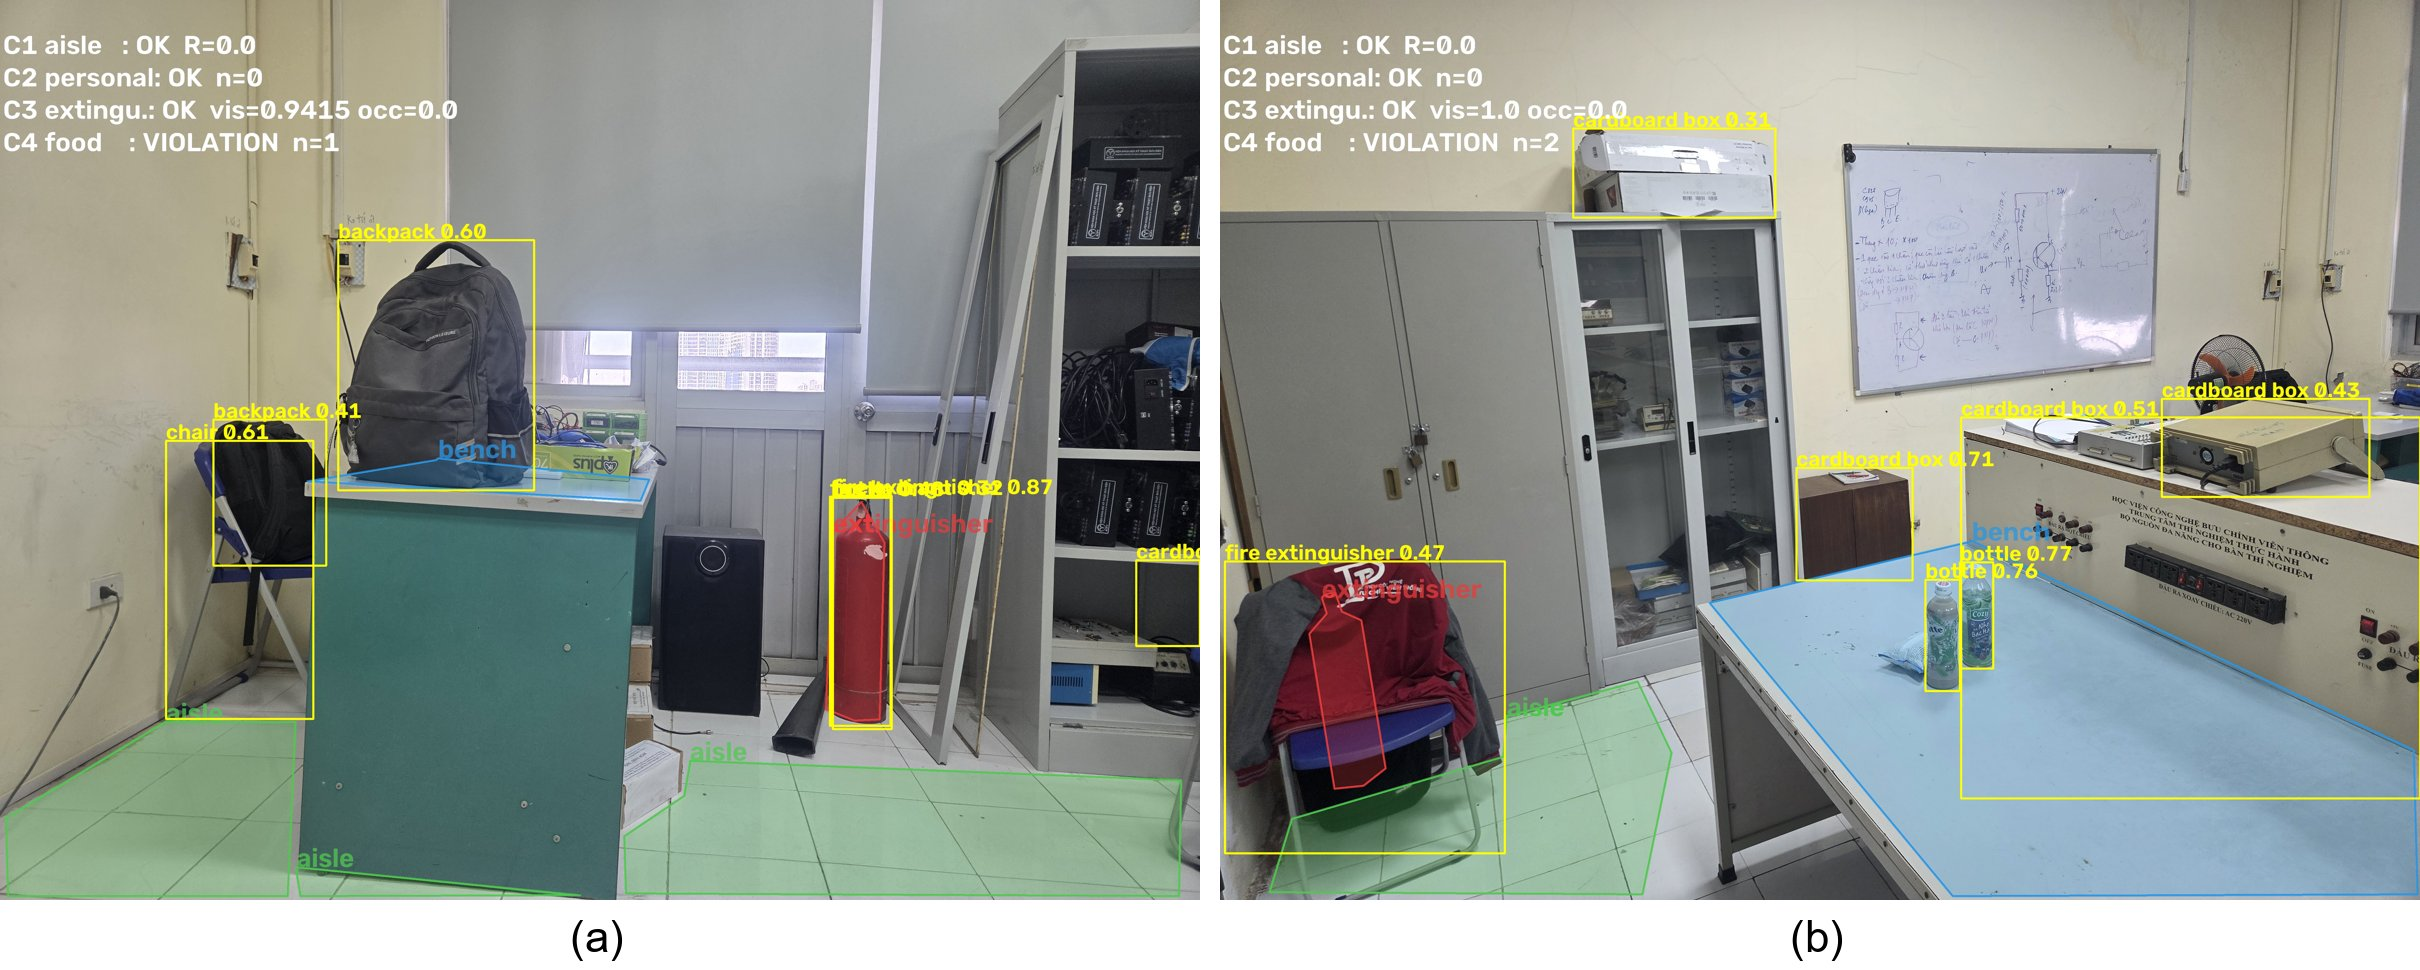
\includegraphics[width=\columnwidth]{fig_errors.jpg}
\caption{Ca lỗi của hệ thống luật. (a) COCO nhận bình chữa cháy thành \emph{bottle} nên C4 báo vi phạm sai. (b) Áo khoác trùm bình không được phát hiện là vật che nên C3 bị bỏ sót.}
\label{fig:errors}
\end{figure}

\subsection{Tốc độ và chi phí}
Hệ thống luật xử lý một ảnh trong khoảng 0{,}13~s (trung vị) trên GPU MX350 2~GB, chạy hoàn toàn cục bộ. VLM cần trung bình 10{,}3~s mỗi ảnh (trung vị 7{,}3~s) qua mạng, với khoảng 1.400 token đầu vào và 110 token đầu ra. Gói miễn phí giới hạn khoảng 20 yêu cầu mỗi ngày cho mỗi tài khoản, đủ cho thử nghiệm nhưng không đủ cho giám sát liên tục.

% =====================================================================
\section{Kết luận và hướng phát triển}
Bài báo so sánh hệ thống dựa trên luật (YOLO kết hợp luật không gian) và mô hình ngôn ngữ--thị giác với ba người chấm trên bốn tiêu chí an toàn phòng thí nghiệm. Cả hai hệ thống đạt mức khớp từ trung bình đến gần như hoàn hảo ở phần lớn tiêu chí (RQ1). Hệ thống luật vượt trội ở các tiêu chí phụ thuộc vị trí (lối đi, bình chữa cháy), trong khi VLM vượt trội ở các tiêu chí cần nhận biết loại đồ vật (vật dụng cá nhân, đồ ăn uống) (RQ2). VLM ổn định theo prompt ở các tiêu chí rõ ràng nhưng dao động ở các tiêu chí cần đếm hoặc xác định phạm vi (RQ3). Kết quả gợi ý một hệ thống lai: dùng luật cho C1, C3 và VLM cho C2, C4.

\textbf{Hạn chế.} (i) Ảnh được dàn dựng theo kịch bản tại một phòng thí nghiệm điện tử duy nhất, chưa phản ánh hoàn toàn điều kiện thực tế; (ii) quy mô dữ liệu nhỏ, C2 chỉ có 11 ca vi phạm nên khoảng tin cậy của $\kappa$ rộng; (iii) P2, P3 chỉ được đánh giá trên 33 ảnh do giới hạn hạn mức API; (iv) luật tính trên mặt phẳng ảnh 2D, chưa hiệu chỉnh phối cảnh, và các ngưỡng được chọn trước, chưa được tối ưu.

\textbf{Hướng phát triển.} Bổ sung hai tiêu chí hóa chất ngoài tủ và dây điện cắt ngang lối đi; thu thập dữ liệu từ camera giám sát thực tế; kết hợp hai hướng, chẳng hạn dùng luật cho tiêu chí đếm được và VLM cho tiêu chí cần hiểu ngữ cảnh.

% =====================================================================
\bibliographystyle{IEEEtran}
\bibliography{refs}

\end{document}
